\documentclass[11pt]{article}






%\usepackage{times}
\usepackage{palatino}%charter}
\usepackage{multirow}
\usepackage{wrapfig}
\usepackage{url}
\usepackage{citesort}
\usepackage{epsfig}
\usepackage{graphicx}
\usepackage{color}
\usepackage{fullpage}
\usepackage{amssymb}
\usepackage{amsmath}
\usepackage{theorem}
%\theoremstyle{remark} 
%\theoremstyle{definition}
%\usepackage{wide}
%\usepackage[ruled, vlined]{algorithm2e}
\usepackage[ruled, vlined, linesnumbered]{algorithm2e}
\usepackage{color}
%\usepackage{hyperref}


\newcommand{\veps}{\varepsilon}
\newcommand{\eps}{\epsilon}
\newcommand{\E}{\mathbf{E}}
\renewcommand{\Pr}{\mathbf{Pr}}
\newcommand{\abs}[1]{\left| #1 \right|}
\newcommand{\norm}[1]{\left\lVert #1 \right\rVert}

\newcommand{\bbR}{\mathbb{R}}
\newcommand{\bbZ}{\mathbb{Z}}
\newcommand{\calC}{\mathcal{C}}
\newcommand{\calI}{\mathcal{I}}
\newcommand{\calM}{\mathcal{M}}
\newcommand{\calK}{\mathcal{K}}
\newcommand{\emRed}[1][]{\textcolor{blue} #1}
\newcommand{\opt}{\text{OPT}}
\newcommand{\knowopt}{{\sc KnowOpt}}
\newcommand{\alg}{\text{ALG}}
\newcommand{\greedy}{{\sc Greedy}~}
\newcommand{\greedyLazy}{{\sc GreedyLazy}~}
\newcommand{\stocGreedy}{{\sc StocGreedy}~}
\newcommand{\baseline}{{\sc BaselineStream}~}
\newcommand{\offline}{{\sc Offline}~}
\newcommand{\sieveStream}{{\sc SieveStream}~}
\newcommand{\randomStream}{{\sc RandomStream}~}
\newcommand{\circuitStream}{{\sc CircuitStream}~}


\newtheorem{theorem}{Theorem}
\newtheorem{protocol}{Protocol}
\newtheorem{lemma}{Lemma}
\newtheorem{claim}{Claim}
\newtheorem{property}{Property}
\newtheorem{fact}{Fact}
\newtheorem{observation}{Observation}
\newtheorem{heuristic}{Heuristic}
\newtheorem{solution}{Solution}
\newtheorem{corollary}{Corollary}
\newtheorem{scheme}{Scheme}
\newtheorem{strategy}{Strategy}
\newtheorem{invariant}{Invariant}
{\theorembodyfont{\rmfamily}
\newtheorem{remark}{Remark}}
{\theorembodyfont{\rmfamily}
\newtheorem{definition}{Definition}}

\DeclareMathOperator*{\argmin}{arg\,min}
\DeclareMathOperator*{\argmax}{arg\,max}


\newcommand{\chensays}[2][]{\textcolor{red} {\textsc{Chen #1:} \emph{#2}}}




\newenvironment{proof}{\trivlist\item[]\emph{Proof:}}%
{\unskip\nobreak\hskip 1em plus 1fil\nobreak$\Box$
\parfillskip=0pt%
\endtrivlist}





\begin{document}

\title{Report: Experimental Study for Submodular Maximization}
\author{Jiecao Chen\\ jiecchen@indiana.edu}
\date{\today}

\maketitle



%----------- start -----------------------
\section{Roadmap}
In this part, we give a experimental study of submodular maximization. 

\section{The Setup}
\label{sec:setup}

\subsection{Submodular Functions}
We mainly consider two type of submodular functions in our experiment.
\paragraph{Set Cover Problem}
In the \emph{set cover problem}, we are given a collection of subsets of a set $E$, i.e. $V = \{C_1, C_2, \ldots, C_n\}$ where each $C_i \subseteq E$. We define a function $f:2^V \rightarrow \bbR$ such that $f(S) = |\cup_{C\in S} C|$. We can interpret $f$ as follow: given $S$ as a subset of $V$, the value of $f(S)$ is the number of distinct elements covered by the sets in $S$.

One can easily verify that $f$ satisfies the diminishing return property thus is a submodular function. Furthermore, it is clear that $f$ is non-decreasing.  Now given the cardinality constraint, we want to solve the following,

$$\argmax_{S\subseteq V: |S|\leq k} f(S).$$

\subsection{Weighted Vertex Function}
Let $G = (V, E, W)$ be a graph where each $v\in V$ has a weight $w_v > 0$. For any $S \subseteq E$, $V(E)$ is the set of vertices of edges in $S$. Let $f: 2^E \rightarrow \bbR$ be a set function with $f(S) =\sum_{v\in V(S)} w_{v}$, then $f$ is submodular. We call $f$ a \emph{weighted vertex function}.



% \subsection{Informative Vector Machine}
% Kernel machines \cite{SS02} are powerful non-parametric learning techniques. Those approaches use kernel trick to reduce non-linear problems to linear tasks that have been well studied. The data set $V = \{x_1, x_2, \ldots, x_n\}$ is represented in a transformed space via a kernel matrix

% \[ K_V = \left( \begin{array}{ccc}
% \calK(x_1, x_2) & \ldots & \calK(x_1, x_n) \\
% \vdots & \ddots & \vdots \\
% \calK(x_n,x_1) & \ldots & \calK(x_n, x_n) \end{array} \right)\] 
% here $\calK: V\times V \rightarrow \bbR$ is the kernel function that is symmetric and positive definite. 

% For large-scale problem, even representing the matrix $K_V$ (which requires $O(n^2)$ space) is prohibited. The common solution to solve this issue is to select a small representative subset $S \subseteq V$ and only work with $K_S$. The question now becomes how to select the subset $S$. One popular way to measure the quality of selected set $S$ is to use \emph{Informative Vector Machine}(IVM) introduced by Laurence et al. \cite{LSH03}. Formally, we define $f: 2^V \rightarrow \bbR$ with
% $$f(S) = \frac{1}{2} \log\det\left( \mathbf{I} + \sigma^{-2} K_S \right)$$
% where $\mathbf{I}$ is the identity matrix and $\sigma > 0$ is a parameter. IVM has a close connection to the entropy of  muti-variable Gaussian distribution \cite{B14} and it is shown in \cite{S04,B14} that $f$ is a submodular function. We can then select the set $S\subset V$ by solving
% $$\argmax_{S:|S|\leq k} f(S).$$

% In our experiment, we use the heat kernel $\calK_h(e1, e2) = \exp\{-\|e_1-e_2\|_2^2/h^2\}$ where $h > 0$ is a parameter.


\subsection{Datasets}
\paragraph{synthetic:} We create $1000$ subsets of $[1000] = \{1, 2, \ldots, 1000\}$ , each subset is randomly constructed as follows: 1) randomly sample an integer $n$ from $[1, 100)$ as the size; 2) randomly sample $n$ elements without replacement from $[1000]$. The {\sc Synthetic } dataset is then a collection of $1000$ sets.


\paragraph{Facebook:} 
The {\sc Facebook} dataset is a friends list collected from Facebook users. This dataset is an undirected graph with $4039$ nodes, $88234$ edges. More information of this dataset can be found in \cite{snapnets} ego-Facebook.  We assign each node its degree as its weight. The original edges are grouped by nodes.

\subsection{Computation Environments}
Due to lack of computation resources, all experiments were run in a personal laptop with $3.7$GB Memory, $119$GB SSD, 1.70GHzx2-Intel Core i5 CPU. The operating system is Linux Mint 7.2 Cinnamon 64-bit. Experiments for distributed part were simulated in \emph{Apache Spark} with standalone mode. 

\subsection{Code} 
Most code (several scripts are missing) for this experiment are available at 
\begin{itemize}
\item \url{https://github.com/jiecchen/SubmodularLib/tree/master/src}~.
\end{itemize}
It contains about $3000$ lines java and python code.

\section{Simple Greedy Algorithms}
\label{sec:greedy}
In this section, we compare three different greedy algorithms in the problem of monotone submodular maximization subject to cardinality constraint. We compare their efficiency (measured by number of value queries) and the quality of solutions they returned.
\subsection{Greedy Algorithms}
Let $V$ be the ground set and $k$ be the cardinality constraint. $ 0 < \eps < 1$ is a parameter to control the error.
\begin{itemize}
\item \greedy is the standard greedy algorithm that gives $(1 - e^{-1})$-approximation.  See Algorithm \ref{algo:greedy} for details.
\item \greedyLazy is the greedy algorithm with the trick of lazy evaluation \cite{M78}. The idea goes as follows: instead of computing $\Delta_f(e|S)$ for each $e\in V\backslash S$ in Line \ref{line:emax} of Algorithm \ref{algo:greedy},  \greedyLazy keeps an upper bound $\rho(e)$ (initially $+\infty$) on the marginal gain sorted in decreasing order (or kept in a heap). In each iteration, the \greedyLazy algorithm evaluates the element on top of the heap and updates its upper bound via $\rho(e) \gets \Delta(e|S)$. If the updated $\rho(e) \geq \rho(e')$ for all other $e'$, submodularity guarantees that $e$ is the element with the largest marginal gain. The \greedyLazy algorithm again gives $(1 - e^{-1})$-approximation.
\item \stocGreedy is a sampling-based greedy algorithm. In each step where we add one new element to the solution, we consider only a small fraction of the remaining elements ($O(\frac{|V|}{k}\log \frac{1}{\eps})$). In the selected portion of elements, we also use lazy evaluation to obtain further speedup. This algorithm gives $(e^{-1} - \eps)$-approximation in expectation. We omit its detailed description.
\end{itemize}

\begin{algorithm}[H]
\DontPrintSemicolon % Some LaTeX compilers require you to use \dontprintsemicolon instead
\KwIn{$V$ the ground set, $f$ the submodular function, $k$ the cardinality constraint}
\KwOut{a set $S \subseteq V$}
$S \gets \emptyset$\;
\While{$|S| < k$} {
  $e \gets \argmax_{e\in V\backslash S, ~S\cup\{e\}\in \calI} \Delta_f(e|S)$\;\label{line:emax}
  $S \gets S\cup \{e\}$\;
}
\Return{$S$}\;
\caption{\greedy for submodular maximization subject to cardinality constraint}
\label{algo:greedy}
\end{algorithm}

\subsection{Results for {\sc Synthetic}}
\begin{figure}[h]
    \centering
    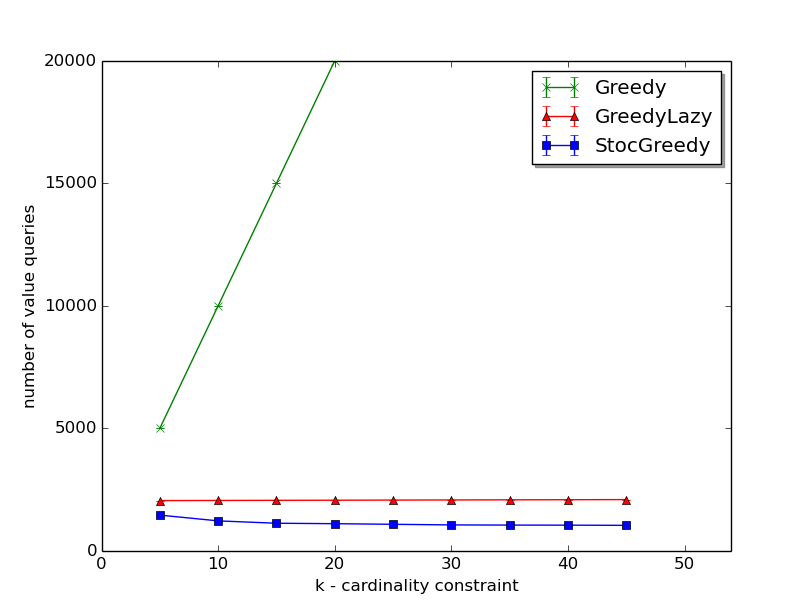
\includegraphics[width=0.5\textwidth]{figures/value-queries.png}
    \caption{Efficiency, measured by number of value queries being used}
    \label{fig:greedy-efficiency}
\end{figure}

\begin{figure}[h]
    \centering
    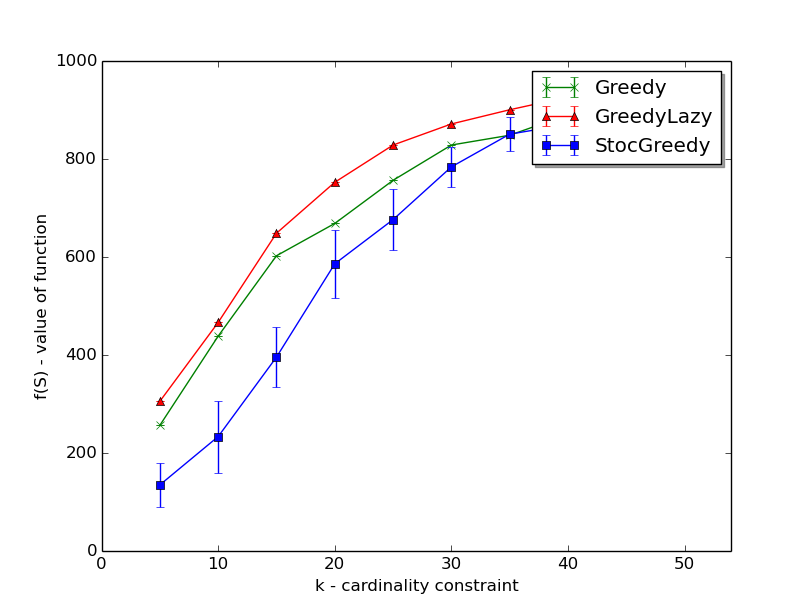
\includegraphics[width=0.5\textwidth]{figures/func-values.png}
    \caption{Quality of Returned Solutions}
    \label{fig:quality-greedy}
\end{figure}



\section{Streaming Submodular Maximization}
\label{sec:streaming}
We compare three different streaming algorithms in the problem of monotone submodular maximization subject to cardinality constraint. In generally it is hard to compare those algorithms fairly because they are configured by different type of parameters. To address this issue, we fixed parameters so that all three algorithms consume roughly the same amount of time. We also compare them with  the standard greedy algorithm (here we call it \offline) and a streaming algorithm (called \baseline) that generates the solution by using random sampling (the notable reservoir sampling is being used internally).


\subsection{Streaming Algorithms}
\begin{itemize}
\item \sieveStream \cite{BMK+14} gives $(1/2 - \eps)$-approximation. See \ref{algo:sieveStream} for details.
\item \randomStream \cite{CGQ15} gives $\frac{1 - \eps}{2 + \eps}$-approximation. See \ref{algo:randomStream} for details.
\item \circuitStream \cite{V11,CGQ15} gives $1/4$-approximation. See \ref{algo:circuitStream} for details.
\end{itemize}
We also compare above three algorithms with \offline and \baseline as mentioned.
\begin{algorithm}[H]
\DontPrintSemicolon % Some LaTeX compilers require you to use \dontprintsemicolon instead
\KwIn{$V$ as data stream, $f$ a monotone submodular function, $k$ the size constraint, $\eps$ a parameter}
\KwOut{a set $S \subseteq V$}
$O = \{(1 + \eps)^i~|~i\in \bbZ\}$\;
\tcc*[h]{maintain the sets only for the necessary $v$'s lazily}\;
For each $v\in O, ~S_v \gets \emptyset$\;
$m \gets 0$\;

\For{each $e$ in the data stream} {
  m $\gets \max\{m, f(\{e\})\}$\;
  $O\gets \{(1 + \eps)^i~|~m \leq (1 + \eps)^i \leq 2\cdot k \cdot m\}$\;
  Delete all $S_v$ such that $v \in O$\;
  \For{$v \in O$}{
    \If{$\Delta(e|S_v) \geq \frac{v/2 - f(S_v)}{k - |S_v|}$ and $|S_v|<k$}{
      $S_v \gets S_v \cup \{e\}$\;
    }
  }
}
\Return{$\argmax_{S_v: v\in O}f(S_v)$}\;
\caption{\sieveStream for submodular maximization}
\label{algo:sieveStream}
\end{algorithm}

\begin{algorithm}[H]
\DontPrintSemicolon % Some LaTeX compilers require you to use \dontprintsemicolon instead
\KwIn{$V$ as data stream, $f$ a non-negative submodular function, $k$ the cardinality constraint, $\eps$ a parameter}
\KwOut{a set $S \subseteq V$}
$B\gets \emptyset, S\gets \emptyset$\;
\For{each $e$ in the data stream} {
  \If{$|S| < k$ and $\Delta(e|S) > \alpha$}{
    $B \gets B + e$\;
  }
  \If{$|B| > \frac{k}{\eps}$}{
    $e \gets $ uniformly random from $B$\;
    $B \gets B - e, S \gets S + e$\;
    \For{all $e'\in B$ s.t. $\Delta(e'|S)\leq \alpha$}{
      $B \gets B - e'$\;
    }
  }
}
$S' \gets$ offline algorithm on $B$\;
\Return{$\argmax_{A\in\{S, S'\}}f(A)$}\;
\caption{\randomStream for submodular maximization}
\label{algo:randomStream}
\end{algorithm}

\begin{algorithm}[H]
\DontPrintSemicolon % Some LaTeX compilers require you to use \dontprintsemicolon instead
\KwIn{$V$ as data stream, $f$ a monotone submodular function, $k$ is the cardinality constraint, $\gamma > 0$ is a parameter}
\KwOut{a set $S \subseteq V$}

\For{each $e$ in the data stream} {
  \If{$|S| < k$}{
    $S \gets S + e$\;
  }
  \Else{
    $e^* \gets \argmin_{e'\in S}f(\{e'\})$\;       
    \If{$f(\{e\}) \geq (1 + \gamma)\cdot f(\{e^*\})$}{
      $S \gets S \cup \{e\} \backslash \{e^*\}$\;
    }  
  }
}
\Return $S$\;
\caption{\circuitStream for  submodular maximization}
\label{algo:circuitStream}
\end{algorithm}



\section{Distributed Submodular Maximization}
\label{sec:distributed}

\section{Discussion and Conclusion}
\label{sec:conclude}



%----------- end -------------------------













\bibliographystyle{abbrv}
\bibliography{survey.bib}

%\newpage

%\appendix
%\input{appendix}


\end{document}
